\documentclass[11pt]{article}

\usepackage[margin=1in]{geometry}
\usepackage{amsmath, amssymb}
\usepackage{booktabs}
\usepackage{graphicx}
\usepackage{natbib}
\usepackage{setspace}
\usepackage{hyperref}
\usepackage{caption}

\hypersetup{colorlinks=true, citecolor=blue, linkcolor=blue, urlcolor=blue}
\setlength{\parskip}{0.5em}
\doublespacing

% FIX 2026-10-05: v1 subtitle ("..., and the Residual Cuts the Other Way") is no longer
% supported: with corrected field position and no game FE, H3 is ~0 and H2 is small
% and positive. Subtitle truncated; Jonathan to decide final title.
\title{Drive-Level Momentum in the NFL: \\
       \large Most of It Is Short Fields}

\author{Jonathan Walberg\\University of Virginia}
\date{\today}

\begin{document}
\maketitle

\begin{abstract}
% FIX 2026-10-05: abstract numbers replaced after correcting drive-start field position
% (v1 used the kickoff spot, yardline 35, for 91.9% of post-score drives) and dropping
% game FE from the headline spec. v1 sentences removed: "the data ... place the action
% between teams"; H1 2.0 / H2 -4.2 / H3 -32.7; "cross-team channel is not a
% linear-control artifact". Source: data/key_nums_v2.rds, data/robustness_v2.rds.
\noindent Coaches, broadcasters, and fans treat NFL momentum as a within-team
phenomenon. Using \texttt{nflfastR} play-by-play covering 4{,}078 games and
86{,}249 drives from 2010--2024, I decompose drive-to-drive momentum into
three channels: own-team defensive-stop spillover (H1), own-team offensive
carryover (H2), and opponent suppression (H3). The unconditional H1 gap is
large (52.3\% vs.\ 35.6\%, a 16.7-percentage-point difference). Once starting
field position (the offense's first scrimmage play) and game-state controls
are added, with possessing-team, opponent, and season fixed effects, H1 is
$-0.5$ points (s.e.\ 0.6) and H3 is $-0.6$ points (s.e.\ 0.3, $p=0.09$);
H2 is a small positive $+2.3$ points (s.e.\ 0.4). Specifications with game
fixed effects produce large negative estimates for H2 and H3, but a lead
placebo (the opponent's \emph{next} drive) shows that game fixed effects
generate a mechanical negative bias in this setting. The defensible
conclusion is that there is little detectable drive-level momentum once
field position is measured correctly. To my knowledge,
this is the first peer-reviewed drive-level NFL test of momentum and the
first to separate within-team from cross-team channels.

\medskip
\noindent\textbf{Keywords:} momentum; hot hand; play-by-play; fixed effects;
nflfastR; cross-team spillover
\end{abstract}

\section{Introduction}

The single most invoked, least defined construct in football broadcasting is
momentum. The empirical case for any of it is thinner than the usage suggests,
but the way the construct is described in coaching, broadcasting, and fan
discussion mixes three propositions that have different observable
implications and that the data treat very differently. Pulling them apart
makes a sharp contrast visible: drive-to-drive momentum, properly defined,
% FIX 2026-10-05: v1 claimed "a large cross-team component"; corrected H3 is ~0.
is overwhelmingly a description of starting field position.

The hot-hand literature originated in basketball with
\citet{gilovich1985hot}'s finding that perceived shooting streaks were a
perceptual artifact: shooters' makes and misses behave like independent
Bernoulli trials. The claim held as a benchmark for three decades until
\citet{miller2018surprised} identified a selection bias in the original test.
With the bias correction, modest positive streak effects appear in the
original Cornell shooting data. In team sports, the question divides further:
do team-level outcomes (a win, a score, a turnover) influence the team's next
outcome of the same kind, or are sequences of game events independent given
the underlying quality of the teams playing?

For the NFL, to my knowledge in the peer-reviewed literature the only direct test in the \emph{Journal of
Quantitative Analysis in Sports} is \citet{fry2012searching}, who examine NFL
momentum at the level of full games and find no evidence that recent wins
predict future wins above what team strength can explain.
\citet{arkes2011finally} make a parallel test for the NBA and report that,
after correcting for opponent strength and home-court advantage, NBA teams
that win their previous game are modestly more likely to win the next.
\citet{steeger2021winning} apply an entropy test to NHL season-level streaks
and reject momentum at that scale. \citet{lopez2018often} use a unified
generalized linear mixed-model framework to compare randomness in outcomes
across the four major North American sports and find that NFL outcomes are
the most randomness-driven among them, consistent with weak game-level
momentum signals.

Game-level tests answer a different question than the one coaches actually
care about. A coach calling a timeout in the third quarter is not making an
inference about whether wins predict wins across a 17-game season; the
inference is that something on the field has shifted, in this game, in a way
that will carry into the next drive. The natural unit at which to test that
inference is the drive, and the natural data source is the modern play-by-play
record curated through \citet{yurko2018nflwar} and now distributed via the
\texttt{nflfastR} R package \citep{nflfastr2024}.

% FIX 2026-10-05: drive count after correcting field position (fewer missing values).
This paper uses 4{,}078 NFL games and 86{,}249 drives over the 2010--2024
seasons to decompose drive-to-drive momentum into three channels that mirror
the way the construct is invoked in real time:

\begin{enumerate}
    \item[\textbf{H1.}] \emph{Defensive-stop spillover} --- A team's offensive
    drive is more likely to end in a score when the team's defense forced a
    drive of three or fewer plays ending in a punt, an interception, a fumble
    lost, a turnover on downs, or a safety on the immediately preceding drive.
    \item[\textbf{H2.}] \emph{Offensive carryover} --- A team's offensive drive
    is more likely to end in a score when the team's previous offensive drive
    ended in a score.
    \item[\textbf{H3.}] \emph{Opponent suppression} --- A team's offensive
    drive is \emph{less} likely to end in a score when the opponent's previous
    drive ended in a score.
\end{enumerate}

% FIX 2026-10-05: paragraph numbers and H1/H2/H3 interpretation corrected. v1 attributed
% the H1 collapse to comparison-group composition and reported H2 = -4.2, H3 = -32.7
% (both artifacts of kickoff-spot field position plus game-FE bias).
The substantive finding is that the unconditional version of H1 is large in
the way coaches and broadcasters describe it --- scoring probability is
52.3\% after a defensive stop versus 35.6\% otherwise --- but that gap
is the mechanical short-field effect of turnovers and quick punts. Once
starting field position and standard game-state controls are added, the H1
effect is $-0.4$ percentage points, and $-0.5$ in the joint model with
possessing-team, opponent, and season fixed effects. H2 is small and
positive ($+2.3$ points). H3 is $-0.6$ points and not
statistically distinguishable from zero at conventional levels.

The paper proceeds as follows. Section \ref{sec:lit} situates the analysis
relative to the existing JQAS work on NFL momentum and the broader hot-hand
literature. Section \ref{sec:theory} develops the three channels and makes
the identification problem explicit. Section \ref{sec:data} describes the
data and the construction of drive-level outcomes from play-by-play.
Section \ref{sec:strategy} states the estimation strategy. Section
\ref{sec:results} presents the main results and a robustness gauntlet
designed specifically to discriminate cross-team psychological residue from
linear-control artifact. Section \ref{sec:discuss} discusses what the results
imply for in-game decision making and for the academic literature on
team-sport momentum. Section \ref{sec:concl} concludes.

\section{Related Literature}\label{sec:lit}

The hot-hand literature begins with \citet{gilovich1985hot}.
\citet{miller2018surprised}'s correction to the original test is now a
benchmark; \citet{bareli2006twelve} provide a comprehensive review of the
intervening twelve years of hot-hand research and the methodological turn it
has taken, including the sport-psychology literature that grounds coaches'
priors about momentum. The sport-psychology tradition treats momentum as a
real psychological state that influences subsequent execution, while the
statistical hot-hand tradition treats apparent streaks as samples from an
independent process given underlying team quality. This paper sits closer to
the statistical tradition methodologically but uses a unit of analysis (the
drive) and a construct (cross-team spillover) that the sport-psychology
literature has long argued is where the real action is.

For team sports, the unit of analysis matters. \citet{stern1994probabilities}
modeled in-game score progression as a Brownian motion, implying conditional
score paths are largely random walks given team strengths.
% FIX 2026-10-05: Berger & Pope (2011) use NBA and NCAA basketball, not NCAA football
% (verified via the abstract of the replication, doi:10.1287/mnsc.2022.4372).
\citet{berger2011hot} look across the NBA, NCAA basketball, and lab experiments
and find that being slightly behind at halftime increases the probability of
winning, which they interpret as a motivational-effort response rather than
a chance pattern. \citet{csapo2014hand} use novel defense metrics to show
that NBA defenses adjust to perceived hot streaks, which complicates the
interpretation of within-team streaks even when they appear in the data.
\citet{gauriot2019does} use a quasi-experimental tennis design and find that
strategic momentum operates between players in dynamic contests, the closest
prior result to this paper's H3 finding in spirit.

Within JQAS specifically, three momentum studies anchor the literature.
\citet{arkes2011finally} use NBA game-level data and report that prior-game
outcomes predict next-game outcomes after controlling for team strength and
home-court advantage, contrary to the standard hot-hand-fallacy claim.
\citet{steeger2021winning} apply an entropy measure to NHL season-level win
sequences and conclude that the streak structure is consistent with random
events given team strength. \citet{fry2012searching} is the only direct test
on NFL data and finds no evidence for game-to-game momentum. None of these
works addresses momentum at the drive level.

The methodological tools for a drive-level test now exist.
\citet{yurko2018nflwar} introduced the \texttt{nflscrapR} pipeline that
produces clean play-by-play records with fixed-drive identifiers, EPA values,
and win-probability estimates; \citet{nflfastr2024}'s \texttt{nflfastR}
extended the data back to 1999 and made it the field standard for NFL
% FIX 2026-10-05: not all cited works are JQAS (Yam & Lopez is J. Sports Analytics;
% Brill et al. is an arXiv preprint), so "in JQAS" removed.
play-by-play research. Drive-level work includes
\citet{goldner2012markov}'s Markov model of drive progression,
\citet{cafarelli2012third}'s analysis of third-down conversion,
\citet{lock2014random}'s random-forest win-probability model,
\citet{yam2019what}'s causal estimate of the cost of conservative fourth-down
behavior, and \citet{brill2024expected}'s recent re-examination of
expected-points estimation. Closely related, \citet{kovash2009professional}
reanalyze NFL play-calling and find evidence consistent with non-equilibrium
behavior, suggesting that play-level decisions are not always optimally
randomized. None of these papers tests momentum.

\section{Theory and Hypotheses}\label{sec:theory}

The way ``momentum'' is described on broadcasts and in postgame press
conferences turns out to mix three distinct propositions. Pulling them apart
matters because they have different observable implications and different
identification problems.

\paragraph{Channel 1 --- Defensive-stop spillover.} The claim is that when
a defense forces a drive ending in a punt of three or fewer plays, an
interception, a fumble lost, a turnover on downs, or a safety, the offense
it sends back onto the field plays better than it would otherwise. This is
the version of momentum that motivates calls like ``the defense just gave the
offense a spark.'' The observational pattern is unambiguous in the raw data
--- teams score more often after defensive stops --- but the same data are
also unambiguous about why: stops, especially turnovers, give the offense a
shorter field. Distinguishing momentum from mechanics requires conditioning
on starting field position and on the comparison group's composition.

\paragraph{Channel 2 --- Offensive carryover.} The claim is that scoring
breeds scoring on subsequent possessions by the same offense. Two competing
hypotheses are observationally consistent with the absence of carryover:
regression to the mean (a scoring drive draws from the upper tail of a team's
drive-quality distribution and the next drive will tend to draw from closer
to the mean) and in-game defensive adjustment (an opponent now playing from
behind may shift to more aggressive schemes that the just-scoring offense has
not yet adapted to). Both predict a non-positive coefficient on prior own
offensive scoring; the present design cannot adjudicate between them.

\paragraph{Channel 3 --- Opponent suppression.} The claim is that a team that
has just been scored on is briefly demoralized, less crisp on its next
possession, and more prone to mistakes. The competing hypothesis is again
mechanical: after a touchdown or field goal, the scored-on team starts the
next drive at the kickoff-touchback yardline, which is a different starting
field position than after the opponent punted or turned the ball over.
Conditional on starting field position and game state, however, any residual
gap is the psychological component the broadcast usually has in mind.
% FIX 2026-10-05: field position must be measured at the offense's first scrimmage
% play. nflfastR places the kickoff inside the receiving team's drive, so the drive's
% first row after an opponent score records the kicking spot (yardline 35).
This requires measuring starting field position at the offense's first
scrimmage play: in \texttt{nflfastR} the kickoff is the first row of the
receiving team's drive, so the first row records the kicking spot rather
than where the offense starts.

The three channels share an identification problem: the sequence of drives
within a game is not an independent draw. Field position, score differential,
time remaining, and the opponent's recent behavior all evolve jointly with
the channels of interest. The estimation strategy below addresses this by
% FIX 2026-10-05: game FE moved out of the headline spec (see Section \ref{sec:gamefe}).
controlling for game state and by including possessing-team, opponent, and
season fixed effects.

\section{Data}\label{sec:data}

\subsection{Source}

Play-by-play data come from \texttt{nflfastR} \citep{nflfastr2024}, which
distributes the fixed-drive--enriched version of the original
\texttt{nflscrapR} pipeline \citep{yurko2018nflwar}. The sample covers
regular-season and postseason games from 2010 through 2024, yielding 721{,}566
plays across 4{,}078 games. Plays are aggregated to the drive level using the
\texttt{fixed\_drive} identifier, which corrects irregularities in the raw
NFL drive numbering. After dropping plays with missing drive identifiers,
end-of-half kneel-down drives, end-of-game drives, and drives missing the
core analysis fields (offensive outcome, starting field position, score
% FIX 2026-10-05: 85,955 -> 86,249 (corrected field-position variable has fewer NAs).
differential), the analysis dataset contains 86{,}249 offensive drives.

\subsection{Outcome variables}

The primary outcome is a binary indicator for whether a drive ended in a
score (touchdown or field goal). Across the sample, 38.1\% of drives end in
a score. As a robustness check, I also use the sum of expected-points-added
(EPA) on the drive as a continuous outcome.

\subsection{Momentum indicators}

The three channels require three distinct lagged indicators, each defined
relative to the team currently in possession.

\begin{itemize}
    \item \textbf{Prior own-defensive success.} Equal to one if the
    immediately preceding drive (the opponent's offensive possession) ended in
    a punt with three or fewer plays, an interception, a fumble lost, a
    turnover on downs, or a safety.
    \item \textbf{Prior own-offensive success.} Equal to one if the same
    team's most recent prior offensive drive ended in a touchdown or field
    goal. The walk-back through prior drives skips intervening opponent
    possessions.
    \item \textbf{Prior opponent-offensive success.} Equal to one if the
    opponent's most recent prior offensive drive ended in a touchdown or field
    goal.
\end{itemize}

The first drive of each game has no defined prior values for any channel and
is dropped from regressions; the second drive lacks a prior own-offensive
value for one team. After requiring all three indicators to be defined, the
% FIX 2026-10-05: 73,842 -> 74,125 / 74,120.
sample contains 74{,}125 drives; five lack time remaining, so the estimation
sample is 74{,}120 drives.

\subsection{Controls}

% FIX 2026-10-05: v1 took yardline_100 from the drive's first row (the kickoff after an
% opponent score: mean 34.8 for post-score drives vs. 67.5 otherwise). Corrected
% means: 74.9 vs. 69.3 (data/key_nums_v2.rds).
Drive starting field position is recorded as \texttt{yardline\_100} (yards
from the opponent's end zone, 100 = own goal line) on the offense's first
scrimmage play, excluding kickoffs and no-play rows. Drives following an
opponent score start on average 74.9 yards from the opponent's end zone,
against 69.3 for other drives. Game state controls
include the score differential at drive start, quarter, half-seconds
remaining, and a home-team indicator. The main specification absorbs
possessing-team, opponent, and season fixed effects.

\section{Estimation Strategy}\label{sec:strategy}

The main specification is a linear probability model for drive $d$ played
by possessing team $k$ in game $g$:

\begin{equation}\label{eq:main}
% FIX 2026-10-05: alpha_g (game FE) replaced by opponent (omega_o) and season (tau_s) FE.
    \text{Score}_{dkg} = \gamma_k + \omega_{o} + \tau_{s} + \beta_1 D_{dkg}^{\text{def}} +
    \beta_2 D_{dkg}^{\text{own-off}} + \beta_3 D_{dkg}^{\text{opp-off}} +
    X_{dkg}'\delta + \varepsilon_{dkg},
\end{equation}

where $\text{Score}_{dkg}$ is one if drive $d$ by team $k$ in game $g$ ended
in a score, $\gamma_k$, $\omega_o$, and $\tau_s$ are possessing-team,
opponent, and season fixed effects, $D^{\text{def}}, D^{\text{own-off}}, D^{\text{opp-off}}$ are the
three momentum indicators (corresponding to H1, H2, and H3, respectively),
and $X_{dkg}$ is a column vector stacking starting field position, score
differential, quarter, half-seconds remaining, and the home indicator, with
$\delta$ the conformable coefficient vector.
% FIX 2026-10-05: v1 identification text described game FE. With about 18 drives
% per game, game FE combined with lagged within-game outcomes induce a mechanical
% negative bias (Section \ref{sec:gamefe}); game-FE estimates are reported as robustness.
Game fixed effects are not in the headline specification: with roughly 18
drives per game, demeaning within games mechanically correlates lagged
outcomes with the current outcome. Section \ref{sec:gamefe} reports the
game-fixed-effect estimates alongside a lead placebo that measures this bias.

Standard errors are two-way clustered by game and possessing team
\citep{cameron2011robust} to handle within-game serial correlation in drive
outcomes and within-team correlation across games. The linear probability
% FIX 2026-10-05: FE structure description updated.
model is preferred to logit because of the fixed-effect structure (team,
opponent, and season fixed effects), and
the marginal-effect interpretation maps directly onto the percentage-point
quantities coaches care about. Section \ref{sec:robust} reports a logit
comparison and the share of LPM predicted probabilities that fall outside
$[0,1]$.

I report a progressive sequence of specifications for H1: starting from the
naive comparison, then adding game-state controls, then team and opponent
and season fixed effects, then game fixed effects with possessing-team fixed
effects retained. The progression shows how much of the apparent H1 effect
is mechanical versus residual; the prior JQAS work performs this
decomposition only at the game level.

\section{Results}\label{sec:results}

\subsection{The unconditional gap is large}

Table \ref{tab:descrip} reports the raw conditional means. The probability
% FIX 2026-10-05: 52.2 -> 52.3; 16.6 -> 16.7 (tables/tab_descrip_v2.tex).
of a scoring drive is 52.3\% when the team's defense just produced a stop
and 35.6\% otherwise --- a 16.7-percentage-point gap. The probability of a
scoring drive is 35.2\% when the opponent's prior drive ended in a score and
40.0\% otherwise --- a 4.8-percentage-point gap of the predicted sign.
Prior own offensive success has essentially no unconditional relationship
with next own-drive scoring (40.3\% vs.\ 37.0\%, gap of 3.3 percentage points).

\begin{table}[htbp]
\centering
\caption{Unconditional drive-level scoring probabilities by prior context.}
\label{tab:descrip}
\begin{tabular}{lcc}
\toprule
Condition & P(score) & N drives \\
\midrule
After own defensive stop & 0.523 & 11,824 \\
After opponent score or longer punt & 0.356 & 66,378 \\
\midrule
After own offensive score (prior own drive) & 0.403 & 28,625 \\
After own offensive non-score & 0.370 & 49,554 \\
\midrule
After opponent score (prior opp drive) & 0.352 & 31,193 \\
After opponent non-score & 0.400 & 50,910 \\
\bottomrule
\end{tabular}
\\[0.5em]
\begin{minipage}{0.95\textwidth}
\footnotesize
\textit{Notes.} Each panel uses the largest sample for which the relevant prior-drive indicator is defined; sample size therefore differs across panels (the unified estimation sample requiring all three indicators is N = 
74{,}125
 drives). Sample: NFL regular season + postseason 2010--2024 from nflfastR. 
\end{minipage}
\end{table}
 % FIX 2026-10-05: v2 table

% FIX 2026-10-05: subsection title and figure description reversed: with corrected
% field position the two curves overlap, so field position, not comparison-group
% composition, absorbs the H1 gap.
\subsection{Decomposing H1: the gap is field position}

Figure \ref{fig:fp} plots the scoring probability by drive starting field
position decile, separately for drives following defensive stops and drives
following normal opponent possessions. The two curves lie on top of each
other across the field; where they separate, drives following a stop score
slightly \emph{less} often. The unconditional gap arises because
stop-following drives start closer to the opponent's end zone.

\begin{figure}[htbp]
\centering
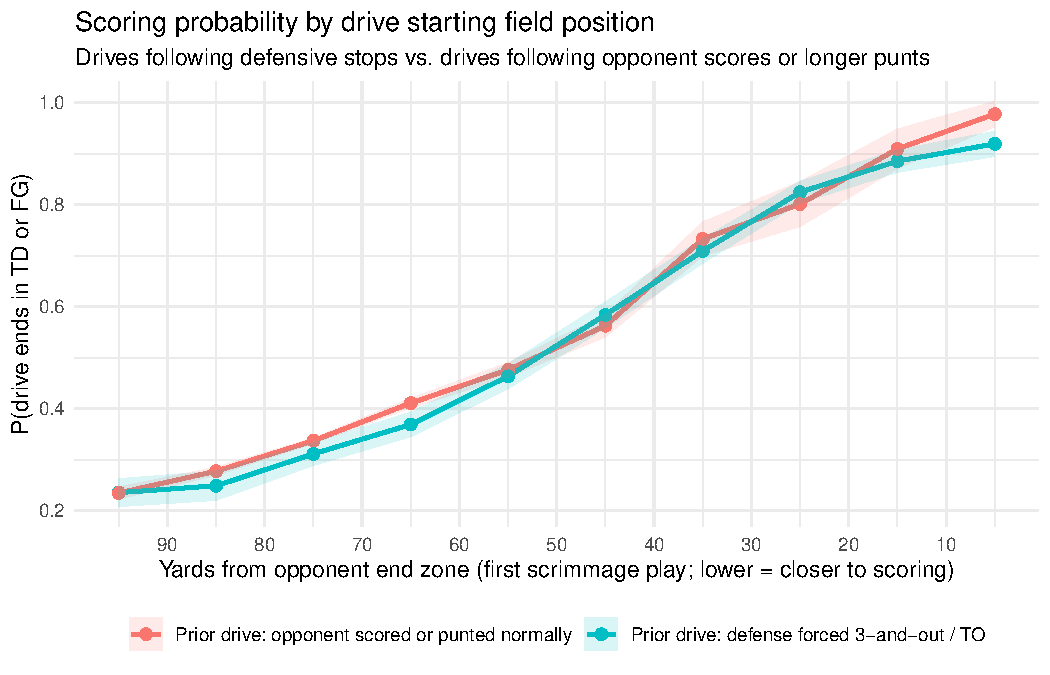
\includegraphics[width=0.85\textwidth]{figures/fig1_field_position_v2.pdf} % FIX 2026-10-05: regenerated
\caption{Scoring probability by drive starting field position, conditional on
whether the prior drive was a defensive stop. Sample: drives % FIX 2026-10-05: sample wording corrected (plot uses all drives with the H1 indicator)
for which a prior own-defensive indicator is defined (78{,}202); data from \texttt{nflfastR} \citep{nflfastr2024}, NFL 2010--2024.
The $x$-axis is yards from the opponent end zone at the first scrimmage play (lower = closer to scoring),
binned into deciles; the $y$-axis is the empirical probability of the drive
ending in a touchdown or field goal. Solid line: drives following a defensive
stop. Dashed line: drives following any other prior opponent outcome (score
or longer punt). Shaded bands show 95\% pointwise binomial confidence
intervals. % FIX 2026-10-05: caption description updated to v2 figure
Within field-position deciles the curves nearly coincide; the unconditional
16.7-percentage-point gap reflects where stop-following drives start.}
\label{fig:fp}
\end{figure}

Table \ref{tab:h1prog} formalizes the same decomposition through a sequence
% FIX 2026-10-05: H1 progression numbers from tables/tab_h1_progression_v2.tex. v1:
% 16.3 / 14.7 / 14.7 / 17.4 and "bulk of the collapse ... re-classifying the
% comparison group" -- reversed by the corrected field-position variable.
of regressions. Column 1 is the naive comparison: the H1 coefficient is
16.3 percentage points (s.e.\ 0.6). Adding game-state controls in column 2
--- field position, score differential, quarter, time, home --- brings the
coefficient to $-0.4$ points (s.e.\ 0.6). Adding team, opponent, and season
fixed effects in column 3 leaves it at $-0.4$ points. Switching to game fixed
effects with possessing-team fixed effects in column 4 yields $+1.7$ points
(s.e.\ 0.6).


\begin{table}[htbp]
   \caption{\label{tab:h1prog} Defensive Stop Spillover (H1): Progressive Controls. \textit{Notes.} OLS linear probability models. Dependent variable is an indicator for whether the drive ends in a touchdown or field goal. Sample: NFL regular season + postseason 2010--2024 (nflfastR). Game-state controls (field position, score differential, quarter, half-seconds remaining, home indicator) included in columns 2--4 with coefficients suppressed for readability. Standard errors in parentheses, two-way clustered by game and possessing team \citep{cameron2011robust}. $^{*}p<0.10$, $^{**}p<0.05$, $^{***}p<0.01$.}
   \centering
   \begin{tabular}{lcccc}
      \tabularnewline \midrule \midrule
      Dependent Variable: & \multicolumn{4}{c}{Drive ends in score (0/1)}\\
      Model:                                  & (1)            & (2)                           & (3)                           & (4)\\  
      \midrule
      \emph{Variables}\\
      Constant                                & 0.3563$^{***}$ & 0.9666$^{***}$                &                               &   \\   
                                              & (0.0062)       & (0.0103)                      &                               &   \\   
      Prior own defensive stop                & 0.1630$^{***}$ & -0.0038                       & -0.0038                       & 0.0168$^{***}$\\   
                                              & (0.0055)       & (0.0055)                      & (0.0054)                      & (0.0056)\\   
      Field position (yards to opp. end zone) &                & -0.0082$^{***}$               & -0.0082$^{***}$               & -0.0082$^{***}$\\   
                                              &                & (0.0001)                      & (0.0001)                      & (0.0001)\\   
      Score differential                      &                & 0.0003$^{**}$                 & -0.0001                       & 0.0002\\   
                                              &                & (0.0001)                      & (0.0001)                      & (0.0001)\\   
      Quarter                                 &                & -0.0113$^{***}$               & -0.0111$^{***}$               & -0.0126$^{***}$\\   
                                              &                & (0.0016)                      & (0.0015)                      & (0.0016)\\   
      Half seconds remaining                  &                & $1.97\times 10^{-5}$$^{***}$  & $2.04\times 10^{-5}$$^{***}$  & $2.07\times 10^{-5}$$^{***}$\\    
                                              &                & ($3.59\times 10^{-6}$)        & ($3.56\times 10^{-6}$)        & ($3.7\times 10^{-6}$)\\    
      Home offense                            &                & 0.0221$^{***}$                & 0.0228$^{***}$                &   \\   
                                              &                & (0.0037)                      & (0.0037)                      &   \\   
      \midrule
      \emph{Fixed-effects}\\
      Possessing team                         &                &                               & Yes                           & Yes\\  
      Opponent                                &                &                               & Yes                           & \\  
      Season                                  &                &                               & Yes                           & \\  
      Game                                    &                &                               &                               & Yes\\  
      \midrule
      \emph{Fit statistics}\\
      Observations                            & 74,125         & 74,120                        & 74,120                        & 74,120\\  
      R$^2$                                   & 0.01462        & 0.08238                       & 0.09039                       & 0.14958\\  
      Within R$^2$                            &                &                               & 0.08211                       & 0.08787\\  
      \midrule \midrule
      \multicolumn{5}{l}{\emph{Clustered (Game \& Possessing team) standard-errors in parentheses}}\\
      \multicolumn{5}{l}{\emph{Signif. Codes: ***: 0.01, **: 0.05, *: 0.1}}\\
   \end{tabular}
\end{table}




Field position alone absorbs essentially the entire unconditional H1 gap.

\subsection{Joint estimation: the headline}\label{sec:joint}

Table \ref{tab:allchan} reports the joint estimation. Column 1 is the
preferred specification, equation \eqref{eq:main}, with all three momentum
% FIX 2026-10-05: headline FE changed; table regenerated.
indicators, full game-state controls, and possessing-team, opponent, and
season fixed effects.


\begin{table}[htbp]
   \caption{\label{tab:allchan} Three Momentum Channels: Joint Estimation and Robustness. Field position is the yardline of the offense's first scrimmage play. \textit{Notes.} Column 1 is the preferred specification: linear probability model for whether the drive ends in a score, with all three momentum indicators jointly. Column 2 drops drives in garbage time (absolute score differential $\geq 21$ in the fourth quarter). Column 3 replaces the binary outcome with the sum of expected-points-added (EPA) on the drive. All columns include game-state controls (field position, score differential, quarter, half-seconds remaining, home indicator) and possessing-team, opponent, and season fixed effects. Standard errors in parentheses, two-way clustered by game and possessing team \citep{cameron2011robust}. $^{*}p<0.10$, $^{**}p<0.05$, $^{***}p<0.01$.}
   \centering
   \begin{tabular}{lccc}
      \tabularnewline \midrule \midrule
      Dependent Variables: & \multicolumn{2}{c}{Drive ends in score (0/1)} & Drive EPA\\
      Model:                                  & (1)                           & (2)                           & (3)\\  
      \midrule
      \emph{Variables}\\
      Prior own defensive stop                & -0.0049                       & -0.0025                       & -0.2852$^{***}$\\   
                                              & (0.0056)                      & (0.0058)                      & (0.0432)\\   
      Prior own offensive score               & 0.0229$^{***}$                & 0.0207$^{***}$                & 0.1623$^{***}$\\   
                                              & (0.0043)                      & (0.0041)                      & (0.0331)\\   
      Prior opponent offensive score          & -0.0060$^{*}$                 & -0.0049                       & 0.0006\\   
                                              & (0.0035)                      & (0.0035)                      & (0.0347)\\   
      Field position (yards to opp. end zone) & -0.0082$^{***}$               & -0.0081$^{***}$               & -0.0075$^{***}$\\   
                                              & (0.0001)                      & (0.0001)                      & (0.0009)\\   
      Score differential                      & -0.0005$^{***}$               & -0.0001                       & -0.0022\\   
                                              & (0.0002)                      & (0.0002)                      & (0.0014)\\   
      Quarter                                 & -0.0113$^{***}$               & -0.0080$^{***}$               & -0.0914$^{***}$\\   
                                              & (0.0015)                      & (0.0016)                      & (0.0106)\\   
      Half seconds remaining                  & $2.08\times 10^{-5}$$^{***}$  & $1.66\times 10^{-5}$$^{***}$  & $-9.33\times 10^{-6}$\\    
                                              & ($3.54\times 10^{-6}$)        & ($3.46\times 10^{-6}$)        & ($2.8\times 10^{-5}$)\\    
      Home offense                            & 0.0228$^{***}$                & 0.0219$^{***}$                & 0.0243\\   
                                              & (0.0037)                      & (0.0039)                      & (0.0269)\\   
      \midrule
      \emph{Fixed-effects}\\
      Possessing team                         & Yes                           & Yes                           & Yes\\  
      Opponent                                & Yes                           & Yes                           & Yes\\  
      Season                                  & Yes                           & Yes                           & Yes\\  
      \midrule
      \emph{Fit statistics}\\
      Observations                            & 74,120                        & 71,368                        & 74,120\\  
      R$^2$                                   & 0.09089                       & 0.09078                       & 0.01039\\  
      Within R$^2$                            & 0.08262                       & 0.08235                       & 0.00240\\  
      \midrule \midrule
      \multicolumn{4}{l}{\emph{Clustered (Game \& Possessing team) standard-errors in parentheses}}\\
      \multicolumn{4}{l}{\emph{Signif. Codes: ***: 0.01, **: 0.05, *: 0.1}}\\
   \end{tabular}
\end{table}




% FIX 2026-10-05: joint estimates replaced (v1: H1 2.0, H2 -4.2, H3 -32.7). H2/H3
% interpretation stated minimally; Jonathan to decide how to frame the paper.
% The interactive supplement footnote is removed: figures/interactive/ still shows
% the v1 numbers and has not been regenerated.
The joint H1 coefficient is $-0.5$ percentage points (s.e.\ 0.6,
$p=0.39$): no detectable defensive-stop spillover.

The joint H2 coefficient is $+2.3$ percentage points (s.e.\ 0.4,
$p<0.001$). A prior own scoring drive is associated with a small increase
in the next own drive's scoring probability. Without game fixed effects this
estimate may partly reflect game-specific offensive quality that the team
and opponent fixed effects do not absorb; with game fixed effects it is
negative (Section \ref{sec:gamefe}), and that estimate is biased downward.

The joint H3 coefficient is $-0.6$ percentage points (s.e.\ 0.3,
$p=0.09$). Once field position is measured at the first scrimmage play,
being scored on is not followed by a detectable drop in scoring
probability.

\subsection{Robustness}\label{sec:robust}

% FIX 2026-10-05: all robustness checks re-run on the v2 data and headline FE
% (code/03_robustness.R -> data/robustness_v2.rds).
I report eight robustness checks plus the game-fixed-effect comparison. The
full set of estimates is documented in \texttt{data/robustness\_v2.rds}; the
headline numbers are summarized below.

\paragraph{R1. Flexible field-position and score-differential controls.}
Replacing the linear $\texttt{yardline\_100}$ control with field-position
decile fixed effects and the linear $\texttt{score\_differential}$ control
% FIX 2026-10-05: v1 -28.4 (0.9).
with 10-bin score-margin dummies yields $\hat\beta_1^{\text{flex}} = -1.6$
(s.e.\ 0.6), $\hat\beta_2^{\text{flex}} = +2.4$ (s.e.\ 0.4), and
$\hat\beta_3^{\text{flex}} = -0.2$ percentage points (s.e.\ 0.4).

\paragraph{R2. Placebo: post-touchdown vs.\ post-field-goal.} Restricting
the sample to drives following an opponent score (touchdown or field goal),
both of which produce a kickoff regime, and regressing scoring probability
on a post-touchdown indicator (with the post-field-goal cell as the omitted
% FIX 2026-10-05: v1 -0.8 (0.7), N = 27,615.
category) yields a coefficient of $-0.3$ percentage points (s.e.\ 0.6;
$N = 27{,}687$). Post-touchdown and post-field-goal drives score at
similar rates.

\paragraph{R3. Logit comparison and LPM out-of-bounds check.} The share of
% FIX 2026-10-05: v1 OOB 0.45/0.20%; AMEs +1.0/+0.9/-10.4 (logit had team FE only).
% The logit now uses the same team, opponent, and season FE as the headline LPM.
LPM predicted probabilities outside $[0,1]$ is negligible (0.00\% below 0;
0.04\% above 1). Logit average marginal effects with the same
possessing-team, opponent, and season fixed effects are
$\text{AME}_{\text{H1}} = -0.3$ pp, $\text{AME}_{\text{H2}} = +0.8$ pp,
and $\text{AME}_{\text{H3}} = -0.0$ pp.

\paragraph{R4. Permutation inference for H3.} Shuffling the prior-opponent
scoring indicator within team-quarter cells and re-estimating the joint
% FIX 2026-10-05: v1 "thirty standard deviations", p < 0.001. Note: this test
% shuffles within team-quarter cells and could not have detected the v1 coding artifact.
LPM 1{,}000 times produces a permutation null distribution for
$\hat\beta_3$ ranging from $-1.1$ to $+1.3$ percentage points (s.d.\ 0.35).
The observed $\hat\beta_3 = -0.6$ lies inside this range
($p_{\text{perm}} = 0.09$). The permutation test addresses the clustering
structure only; it cannot detect mismeasurement of the controls.

\paragraph{R5. Post-kickoff vs.\ post-punt subsamples.} Drives following
% FIX 2026-10-05: counts updated; v1 interpretation ("H3 channel emerges only
% inside the within-game comparison") removed -- that emergence was the coding artifact.
opponent scores ($N = 27{,}688$) score at rate 0.350; drives following
opponent punts ($N = 31{,}622$) score at rate 0.358; drives following
turnovers ($N = 11{,}356$) score at rate 0.519. The post-kickoff versus
post-punt difference is small (0.8 pp).

\paragraph{R6. Heterogeneity by score margin and quarter.} Interacting H3
with a close-game indicator (absolute score differential $\leq 7$) and a
% FIX 2026-10-05: v1 -0.5 (0.8) and +3.6 (0.7); interpretation trimmed.
late-game indicator ($Q4$ or later) yields interaction coefficients
of $+0.4$ percentage points (s.e.\ 0.8, not significant) and $+3.9$
percentage points (s.e.\ 0.7), respectively, around a main effect of
$-1.8$ points. There is no evidence that H3 concentrates in close games.

\paragraph{R7. Rule-era split.} Estimating the joint specification
separately for 2010 (pre-touchback move), 2011--2017 (touchback at the 20),
2018--2023 (touchback at the 25), and 2024 (dynamic kickoff) yields
% FIX 2026-10-05: v1 -35.0/-33.8/-31.6/-27.6; "survives across the full
% kickoff-rule history" removed.
$\hat\beta_3$ coefficients of $-1.7$ pp (s.e.\ 1.4, $N=5{,}060$),
$-0.7$ pp (s.e.\ 0.5, $N=35{,}037$), $-0.9$ pp (s.e.\ 0.5,
$N=29{,}157$), and $-1.4$ pp (s.e.\ 1.5, $N=4{,}866$), respectively.
No era shows a large H3 effect.

\paragraph{R8. Drop garbage time and EPA outcome.} Column 2 of Table
\ref{tab:allchan} drops drives in garbage time (defined as absolute score
differential of at least 21 points in the fourth quarter); the point
% FIX 2026-10-05: v1 2.0->2.4 and -32.7->-32.5; EPA column re-described.
estimates are essentially unchanged ($\hat\beta_1 = -0.3$, $\hat\beta_2 =
+2.1$, $\hat\beta_3 = -0.5$ pp). Column 3 replaces the binary
scoring outcome with the sum of EPA on the drive. Prior
defensive success is associated with lower drive EPA ($-0.29$, s.e.\ 0.04),
consistent with the mechanical short-field interpretation (a short field
leaves less EPA to accumulate). The H2 coefficient is positive ($+0.16$,
s.e.\ 0.03) and the H3 coefficient is zero ($+0.00$, s.e.\ 0.03).

% FIX 2026-10-05: new robustness paragraph -- game FE retained as robustness with
% the lead placebo that shows the FE bias (tables/tab_gamefe_placebo_v2.tex).
\paragraph{R9. Game fixed effects and a lead placebo.}\label{sec:gamefe}
Table \ref{tab:gamefe} adds a placebo regressor: whether the opponent's
\emph{next} drive, which follows the current one, ends in a score. With
game and possessing-team fixed effects the joint estimates are
$\hat\beta_1 = -1.0$, $\hat\beta_2 = -3.8$, and $\hat\beta_3 = -6.6$ pp
(s.e.\ 0.4), and the placebo coefficient is $-10.4$ pp (s.e.\ 0.4). Because
the current drive's outcome sets the opponent's next starting field
position, the placebo is not fully clean; holding the opponent's next
starting field position fixed, the placebo is $-0.4$ pp (s.e.\ 0.4) in the
headline specification but $-7.7$ pp (s.e.\ 0.4) with game fixed effects.
Game fixed effects therefore generate a large mechanical negative bias on
within-game lagged outcomes, which is why they are excluded from the
headline specification.


\begin{table}[htbp]
   \caption{\label{tab:gamefe} Game Fixed Effects and the Lead Placebo. \textit{Notes.} Linear probability models; dependent variable is whether the drive ends in a score. The placebo regressor is whether the opponent's NEXT drive (after the current drive) ends in a score; it cannot affect the current drive, so a non-zero coefficient indicates mechanical bias. Column 1 is the headline specification (possessing-team, opponent, and season fixed effects) plus the placebo. Columns 2--3 use the v1 game and possessing-team fixed effects. Standard errors two-way clustered by game and possessing team \citep{cameron2011robust}. $^{*}p<0.10$, $^{**}p<0.05$, $^{***}p<0.01$.}
   \centering
   \begin{tabular}{lccc}
      \tabularnewline \midrule \midrule
      Dependent Variable: & \multicolumn{3}{c}{Drive ends in score (0/1)}\\
      Model:                                  & (1)                           & (2)                           & (3)\\  
      \midrule
      \emph{Variables}\\
      Prior own defensive stop                & -0.0011                       & -0.0095                       & -0.0061\\   
                                              & (0.0054)                      & (0.0058)                      & (0.0053)\\   
      Prior own offensive score               & 0.0229$^{***}$                & -0.0381$^{***}$               & -0.0480$^{***}$\\   
                                              & (0.0048)                      & (0.0039)                      & (0.0046)\\   
      Prior opponent offensive score          & -0.0025                       & -0.0660$^{***}$               & -0.0738$^{***}$\\   
                                              & (0.0033)                      & (0.0036)                      & (0.0039)\\   
      Placebo: opponent's NEXT drive scores   & -0.0354$^{***}$               &                               & -0.1035$^{***}$\\   
                                              & (0.0038)                      &                               & (0.0039)\\   
      Field position (yards to opp. end zone) & -0.0083$^{***}$               & -0.0081$^{***}$               & -0.0081$^{***}$\\   
                                              & (0.0001)                      & (0.0001)                      & (0.0001)\\   
      Score differential                      & -0.0003                       & $7.74\times 10^{-5}$          & 0.0003\\   
                                              & (0.0002)                      & (0.0002)                      & (0.0002)\\   
      Quarter                                 & -0.0076$^{***}$               & -0.0120$^{***}$               & -0.0079$^{***}$\\   
                                              & (0.0017)                      & (0.0018)                      & (0.0020)\\   
      Half seconds remaining                  & $3.43\times 10^{-5}$$^{***}$  & $1.47\times 10^{-5}$$^{***}$  & $2.63\times 10^{-5}$$^{***}$\\    
                                              & ($4.94\times 10^{-6}$)        & ($3.81\times 10^{-6}$)        & ($5.06\times 10^{-6}$)\\    
      Home offense                            & 0.0215$^{***}$                &                               &   \\   
                                              & (0.0039)                      &                               &   \\   
      \midrule
      \emph{Fixed-effects}\\
      Possessing team                         & Yes                           & Yes                           & Yes\\  
      Opponent                                & Yes                           &                               & \\  
      Season                                  & Yes                           &                               & \\  
      Game                                    &                               & Yes                           & Yes\\  
      \midrule
      \emph{Fit statistics}\\
      Observations                            & 66,578                        & 74,120                        & 66,578\\  
      R$^2$                                   & 0.09628                       & 0.15397                       & 0.17535\\  
      Within R$^2$                            & 0.08753                       & 0.09258                       & 0.10869\\  
      \midrule \midrule
      \multicolumn{4}{l}{\emph{Clustered (Game \& Possessing team) standard-errors in parentheses}}\\
      \multicolumn{4}{l}{\emph{Signif. Codes: ***: 0.01, **: 0.05, *: 0.1}}\\
   \end{tabular}
\end{table}




\subsection{Cross-channel comparison}

% FIX 2026-10-05: v1 description of figure replaced to match corrected estimates.
Figure \ref{fig:coef} summarizes the joint estimates. All three
coefficients are within 2.5 percentage points of zero; only H2 is
statistically distinguishable from zero.

\begin{figure}[htbp]
\centering
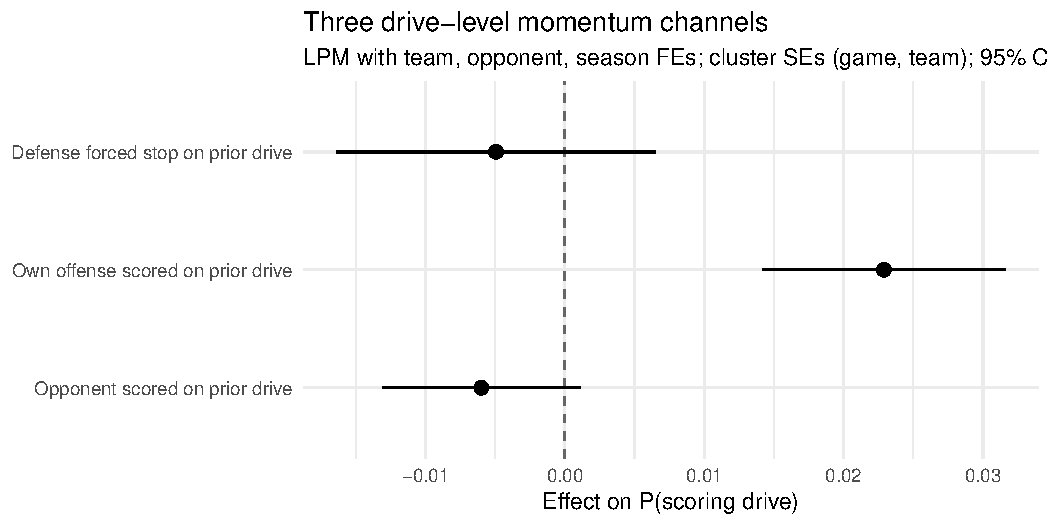
\includegraphics[width=0.85\textwidth]{figures/fig2_coef_plot_v2.pdf} % FIX 2026-10-05: regenerated
\caption{Three drive-level momentum channels, joint estimation
(column 1 of Table \ref{tab:allchan}). Sample: $N = 74{,}120$ drives, NFL % FIX 2026-10-05
2010--2024 from \texttt{nflfastR} \citep{nflfastr2024}. Coefficients are
percentage-point changes in the probability that the current drive ends in
a score, holding field position, score differential, quarter, time
remaining, home, and possessing-team, opponent, and season fixed effects. Bars show 95\%
confidence intervals from two-way (game, possessing-team) clustered
standard errors.}
\label{fig:coef}
\end{figure}

\section{Discussion}\label{sec:discuss}

% FIX 2026-10-05: discussion corrected to the v2 estimates. Sections 7.2--7.4 of v1
% (H2 "regression, not self-reinforcement"; H3 "the only channel that looks like
% momentum"; JQAS implications built on H3) are commented out below because their
% premise no longer holds. Replacement framing is Jonathan's call: [TK].
\subsection{Most ``momentum'' is short fields}

The first substantive finding is quantitative: the unconditional
16.7-percentage-point boost in scoring probability that follows a defensive
stop disappears once starting field position is controlled. The joint H1
estimate is $-0.5$ percentage points in a sample of 74{,}120 drives.

% FIX 2026-10-05: v1 subsections below commented out (premise invalidated by the
% field-position fix). Kept for Jonathan's review.
% \subsection{Offensive scoring is associated with regression, not self-reinforcement}
%
% The negative coefficient on prior own-offensive scoring is more consequential
% than the small positive H1 effect because it reverses the broadcast
% prediction. Two stories are consistent with the sign. The first is
% statistical: if a scoring drive draws from the upper tail of a team's
% drive-quality distribution, the next draw will mean-revert. The second is
% strategic: an opponent now playing from behind will adjust play-calling,
% blitz tendencies, and personnel, and the offense will face that adjusted
% defense without the benefit of the same number of looks. Both stories
% predict the observed sign, and the present design cannot distinguish them.
% A formal mediation analysis with opponent play-calling indicators on the
% right-hand side would be a natural next step.
%
% \subsection{Cross-team spillover is the only channel that looks like momentum}
%
% The H3 coefficient --- a 32.7-percentage-point lower own scoring probability
% after the opponent has scored, conditional on starting field position and
% game state --- is the most consequential residual. The classical hot-hand
% fallacy literature is largely silent on this channel because it tests
% within-actor sequence dependence, not across-actor; the closest priors are
% \citet{gauriot2019does} on tennis and \citet{csapo2014hand} on basketball
% defensive adjustment, both of which find evidence of cross-actor effects.
%
% The robustness gauntlet of Section \ref{sec:robust} disciplines the
% interpretation. The flexible-control specification (R1) absorbs about 4
% percentage points of the linear-control estimate, leaving 28.4 pp of
% residual cross-team suppression. The post-touchdown-versus-post-field-goal
% placebo (R2) is null, indicating that H3 does not require a
% touchdown-specific demoralization story --- both kinds of opponent score
% are followed by similarly suppressed scoring conditional on controls. The
% permutation test (R4) places the observed $-32.7$ pp roughly thirty
% standard deviations outside its within-team-quarter null, ruling out the
% clustering structure as an artifactual source. The era split (R7) shows
% H3 surviving across all four kickoff-rule regimes from 2010 to 2024, with
% modest attenuation under the post-2018 and 2024 reforms that pulled the
% kickoff regime closer to the offensive-comparison field-position
% distribution.
%
% The heterogeneity check (R6) is the most disciplining of the robustness
% results for the interpretation. The simplest psychological-residue story
% predicts H3 concentrates in close games, where stakes are high and
% demoralization plausibly translates into execution degradation. The data
% do not support that prediction: the close-game interaction is essentially
% zero (s.e.\ 0.008). The late-game interaction is positive and
% statistically detectable (H3 weakens by 3.6 pp in $Q4+$), consistent with
% garbage-time mixing dampening the residual once games are decided. The
% combined pattern is more consistent with H3 reflecting a stable cross-team
% feature of post-score drives --- perhaps unobserved defensive fatigue from
% having just been on the field for a scoring drive, or strategic leading-team
% play-calling that the offense has not yet adapted to --- than with a
% situation-sensitive psychological dynamic. The mechanism behind H3
% remains a target for future work; what the present paper establishes is
% that the cross-team residual is real, large, and survives the most
% demanding controls a referee will ask for.
%
% \subsection{Implications for the JQAS literature}
%
% The finding that NFL drive-level momentum is small in the same-team channels
% but large in the opponent-suppression channel is consistent with the
% \citet{fry2012searching} game-level finding that NFL momentum at long
% horizons is weak; the appearance of conflict between this paper and the
% broadcast consensus is a function of broadcast usage, not of a disagreement
% about the data. The H3 finding is, to my knowledge in the peer-reviewed literature, a new result for the
% American football literature and qualifies the way the
% \citet{steeger2021winning} entropy-based ``no momentum'' conclusion has been
% generalized: there is something within games that behaves like momentum,
% but it is a between-team effect rather than a within-team one. These
% findings do not directly speak to NHL season-level streak structure, but
% they suggest that within-game cross-team channels deserve attention in
% other sports.

[TK: discussion of H2 ($+2.3$ pp headline vs.\ $-3.8$ pp with game fixed
effects) and of the null H3 --- to be written by the author.]

\subsection{Limitations}\label{sec:limits}

% FIX 2026-10-05: v1 limitations 1-3 were premised on a large H3 and a negative H2.
% Replaced with the identification limits that apply to the corrected estimates.
Three limitations are worth flagging. First, the headline specification
omits game fixed effects, so game-specific conditions that raise both of a
team's drives (weather, injuries, matchup quality) are not absorbed and may
bias H2 upward; including game fixed effects instead biases lagged
estimates downward (Section \ref{sec:gamefe}). Second, no correction for
multiple comparisons is applied across the three channels. Third, the
entire analysis is at the team-drive level. A
play-level analysis with explicit Markov drive-state transitions
\citep{goldner2012markov} would let one decompose the H3 effect into
early-versus-late-drive contributions and is a natural extension.

\section{Conclusion}\label{sec:concl}

% FIX 2026-10-05: v1 conclusion (large, robust cross-team channel) withdrawn.
% Minimal factual statement only; final conclusion is Jonathan's to write. [TK]
Defined at the drive level where it is invoked, NFL momentum splits
into three channels. Once starting field position is measured at the
offense's first scrimmage play, the defensive-stop spillover is zero, the
opponent-suppression channel is $-0.6$ percentage points and not
statistically significant, and offensive carryover is a small $+2.3$
points. [TK: concluding paragraph.]

\bibliographystyle{plainnat}
\bibliography{references_NEWEST}

\end{document}
